\documentclass[11pt]{article} % set font size to 12
\usepackage[utf8]{inputenc}
\usepackage{indentfirst} % indent first paragraph
\setlength{\parskip}{1em} % line spacing between paragraphs
\setlength{\parindent}{0em} % paragraph indentation
\usepackage[margin=0.75in]{geometry} % set custom margins
\usepackage{amsmath} % for math equations
\usepackage{ amssymb } % for math symbols
\usepackage{graphicx} % for images
\usepackage{wrapfig} % for wrapped images
% Allows us to have clickable references. This should be the last package to be imported!
\usepackage{hyperref}

\title{Experimentation With RL Algorithms}
\author{}
\date{}

\begin{document}
\maketitle

\tableofcontents

\newpage

\section{Introduction}
This writeup focuses on summaries of reinforcement learning (RL) algorithms, and notable implementation details of them. The implementation of algorithms described in this document can be found in \url{https://github.com/leeming99/RL}

We will be skipping explanation on tabular model-based and model-free RL algorithms, which includes Value Iteration, Policy Iteration, Sarsa and Q-learning. Implementations of these algorithms can be found in their respective folders.
% \subsubsection{Model-based RL}
% In fully model-based RL, the most common algorithms are Value Iteration and Policy Iteration, both of which relies on solving the RL problem using dynamic programming in an iterative fashion.
% \subsubsubsection{Value Iteration}
% For value iteration, the idea is that we iterati
\section{Algorithms}
\subsection{Vanilla Policy Gradient (REINFORCE)}
The goal of policy gradient based algorithms is to find parameter $\theta$ that maximizes our objective function:
\begin{equation*}
    J(\theta) = E_{\pi_\theta}\,[log\,\pi_\theta(s,a)\: Q^{\pi_\theta}(s,a)]
\end{equation*}
\begin{figure}
    \centering
    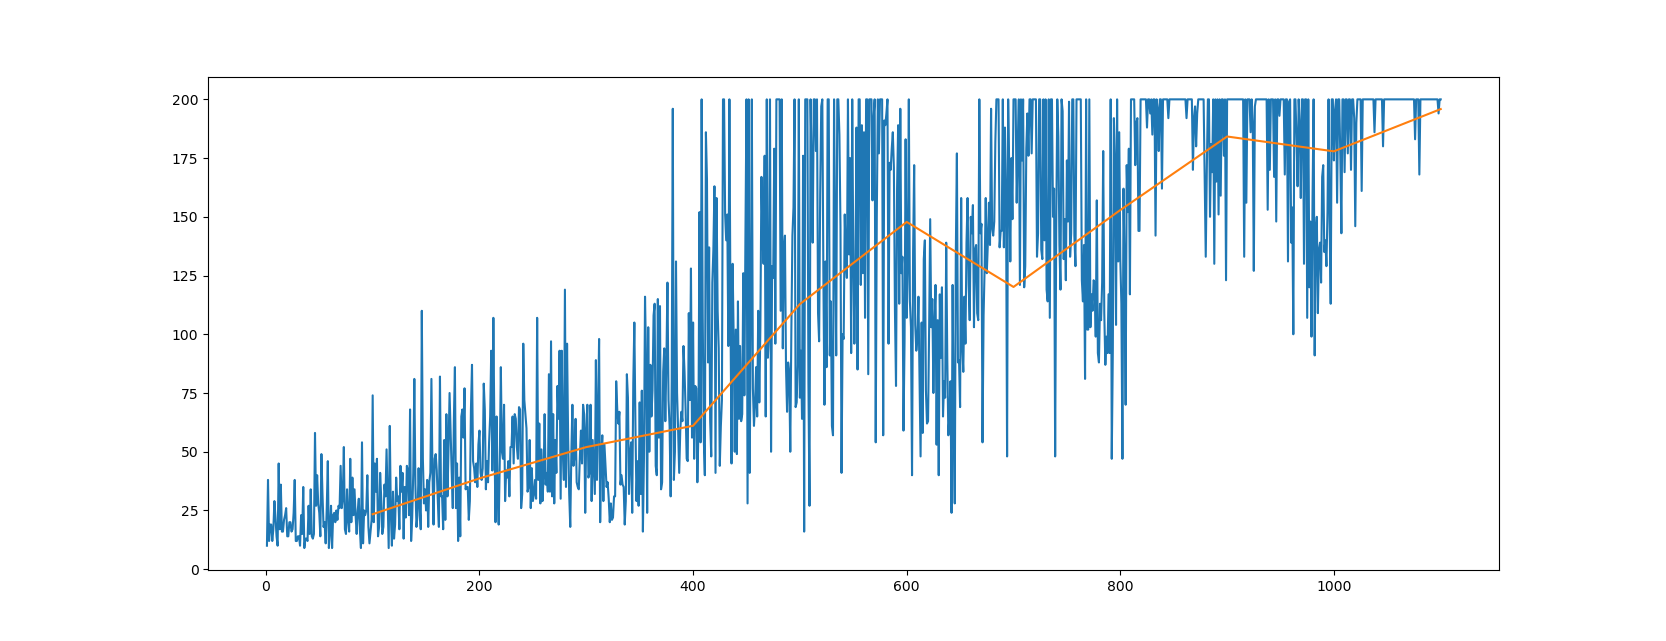
\includegraphics[width=0.7\textwidth]{vanilla_policy_gradient/Solved_cartpole_1100eps.png}
    \caption{Cartpole environment solved in 1100 episodes using REINFORCE}
    % \label{fig:my_label}
\end{figure}
The REINFORCE algorithm \cite{reinforce} optimizes the policy directly, using the discounted cumulative return, $R_t = \sum_{l=0}^\infty \gamma^l r_{t+l}$ as the best estimate of $Q^{\pi_\theta}(s,a)$. Relying on $R_t$ as our estimate of $Q^{\pi}(s,a)$ gives us a low bias but high variance estimate. 

\subsection{Deep Q-Network (DQN)}
DQN uses Q-learning, but with a value function approximator (commonly a deep neural network) instead of a table. The loss function that we try to minimize for is as follows:
\begin{equation*}
    \mathcal{L}_i(w_i) = E_{s, a, r, s'}[(r + \gamma\,max_{a'}Q(s', a'; w_i^-) - Q(s, a; w_i))^2]
\end{equation*}
DQN works because of:
\begin{itemize}
    \item Experience replay buffer - this allows us to be a lot more sample efficient 
    \item Fixed Q-targets - stability during training is achieved by maintaining two different versions of the network (new and old), where we update our new network (which is also our current network) using TD target from our old network. 
\end{itemize}
\subsubsection{Double DQN}
This improvement allows us to reap the benefits from double Q-learning, such as mitigating maximization bias.

Our update function in this case becomes:
\begin{equation*}
    \mathcal{L}_i(w_i) = E_{s, a, r, s'}[(r + \gamma\,Q(s', argmax_{a'}Q(s', a'; w_i); w^-) - Q(s, a; w_i))^2]
\end{equation*}

\subsubsection{Dueling Architecture}
The dueling architecture introduces two separate streams sharing the same network, where one of them outputs $V(s)$, while the other outputs $A(s,a)$ for all actions (see figure \ref{fig:duelingarch}).

\begin{wrapfigure}{r}{0.3\textwidth}
  \begin{center}
    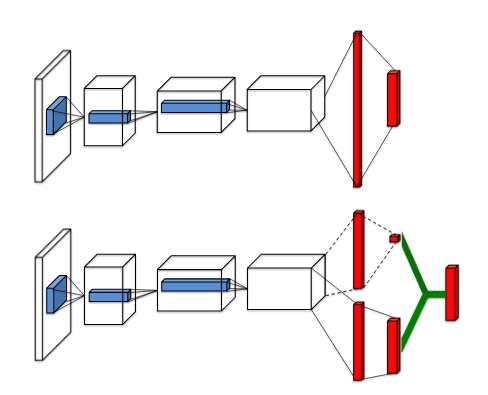
\includegraphics[width=0.3\textwidth]{images/duelingarch.png}
  \end{center}
  \caption{Dueling Architecture from original paper}
  \label{fig:duelingarch}
\end{wrapfigure}

The main idea is that it may not always be important to know the value of every action given a state; rather they are only important when they determine a course of action.

The only modification required is to the output of our network, where 
\begin{equation*}
    Q(s,a;\theta,\alpha,\beta) = V(s; \theta, \beta) + (A(s,a,;\theta,\alpha) - \frac{1}{|A|}\sum_{a'}\, A(s,a';\theta,\alpha))
\end{equation*}

\begin{figure}
    \centering
    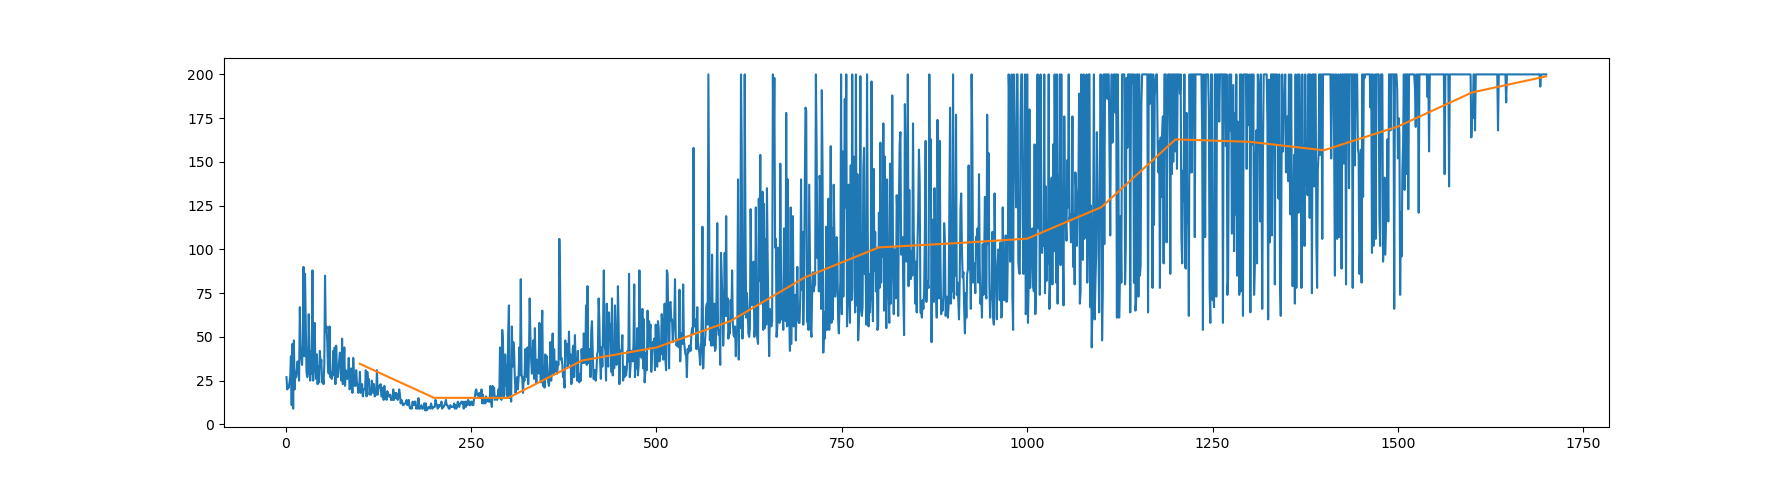
\includegraphics[width=0.8\textwidth]{DQN/Dueling-Double_w_ER_FixedQ/cartpole/1700eps_cartpole.png}
    \caption{DDQN with Dueling Architecture solved Cartpole in 1700 episodes}
    \label{fig:my_label}
\end{figure}

\subsubsection{Prioritized Experience Replay}
Vanilla DQN uniformly samples from the experience replay buffer, which is not ideal since it may not always pick the most valuable information to learn from (i.e. largest TD error $\delta$).

PER solves this by assigning every sample with a priority value, $p$, where $p_i = |\delta_i| + \epsilon$, and the probability of picking sample $i$ is
\begin{equation*}
    P(i) = \frac{p_i^\alpha}{\sum_k p_k^\alpha}
\end{equation*}
To reduce bias caused by sampling high priority experiences more than lower priority ones, we use importance-sampling (IS) weights
\begin{equation*}
    w_i = (\frac{1}{N}\frac{1}{P(i)})^\beta
\end{equation*}

\subsection{Actor Critic Methods}
Using $R_t$ as seen in REINFORCE gives a true value estimation of $Q(s,a)$ and thus is low in bias, but episodic rollouts have a high variance, making its performance often poor.

Value-function approximation methods like DQN estimates $Q(s,a)$ with lower variance (from bootstrapping), but as a result introduces bias. 

Merging both of these, our critic learns a value function, while our actor learns a stochastic policy, such that $\Delta\theta = \alpha \nabla_\theta\, log\, \pi_\theta (s,a)\, Q_w(s,a)$, where $Q_w(s,a)$ is provided by the critic
\subsubsection{Reducing variance with baseline}
To reduce variance of $Q_w(s,a)$, we subtract a baseline function, $b(s)$, from $Q_w(s,a)$. Note that $b(s)$ must not be a function of action (i.e. $b(s,a)$) so that our expectation does not change (i.e. $E_{\pi_\theta}[\nabla_\theta\,log\pi_\theta(s,a)(Q_w(s,a)-b_w(s)] \equiv E_{\pi_\theta}[\nabla_\theta\,log\pi_\theta(s,a)Q_w(s,a)]$.

A good baseline is the state value function $b(s)=V^\pi_\theta(s)$, such that $A^\pi_\theta(s,a) = Q^\pi_\theta(s,a) - V^\pi_\theta(s)$. Since $Q^\pi_\theta(s,a)=r+\gamma V(s')$, we realize that our advantage function can be our TD error $\delta$.

\subsection{A3C \& A2C}
Problems that A3C tries to solve:
\begin{itemize}
    \item Highly correlated data (e.g. frames from video games) meant that neural networks suffer from high variance, and thus converges poorly.
    \item Experience replay buffers use more memory and computation, and limits only to offline algorithms (where data can first be decorrelated).
\end{itemize}
Key ideas that A3C introduces:
\begin{itemize}
    \item Shared architecture between the actor and the critic
    \item Update on fixed-length segments of experience (forward-view n-step TD)
    \item Parallel worker threads, each with separate instances of the environment help decorrelate data
\end{itemize}

\begin{figure}
    \centering
    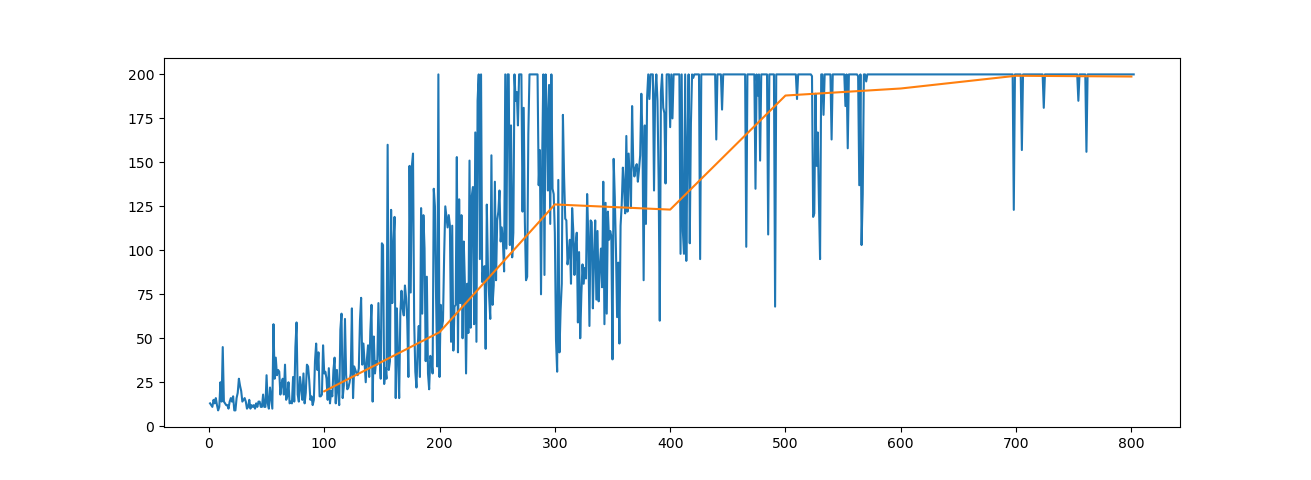
\includegraphics[width=0.8\textwidth]{A3C/cartpole-MC/cartpole_800eps.png}
    \caption{Cartpole environment solved in 800 episode using A3C, running on 4 parallel workers.}
    \label{fig:my_label}
\end{figure}

\subsubsection{Difference between A2C \& A3C}
The major difference between them is that for A3C, worker threads update the main, shared network in an asynchronous fashion, while A2C waits for all actors to complete their segments, before updating the main network, by taking the average over all actors.

A2C is shown to be able to utilize GPUs better (larger batch size), and prevents worker threads from using older versions of the main network.

\subsection{PPO - Proximal Policy Optimization}
Similar to TRPO, PPO is motivated by the question - how can we take the largest improvement step on a policy using a data without causing performance collapse? PPO introduces 2 main ideas:
\begin{enumerate}
    \item \textbf{Clipped Surrogate Objective}\\
    Similar to TRPO, our objective function is 
    \begin{equation*}
    \begin{split}
        J(\theta) &= E_t[\frac{\pi_\theta(a_t|s_t)}{\pi_{\theta_{old}}(a_t|s_t)}A_t] \\
        &= E[r_t(\theta)A_t]
    \end{split}
    \end{equation*}
    The difference is that while TRPO uses KL Divergence constraints to limit $r(\theta)$, PPO uses the Clipped Surrogate Objective
    \begin{equation*}
        J(\theta) = E_t\;[min\,(r_t(\theta)\,A_t, \: clip\,(r_t(\theta),\, 1-\epsilon,\, 1+\epsilon)A_t)]
    \end{equation*}
    \item \textbf{Multiple Epochs Policy Update}\\
    Since our objective function is essentially clipped, this enables PPO to perform gradient ascend on the policy multiple epochs per iteration, without taking steps that are too large. This increases sampling efficiency.
\end{enumerate}
\begin{figure}
    \centering
    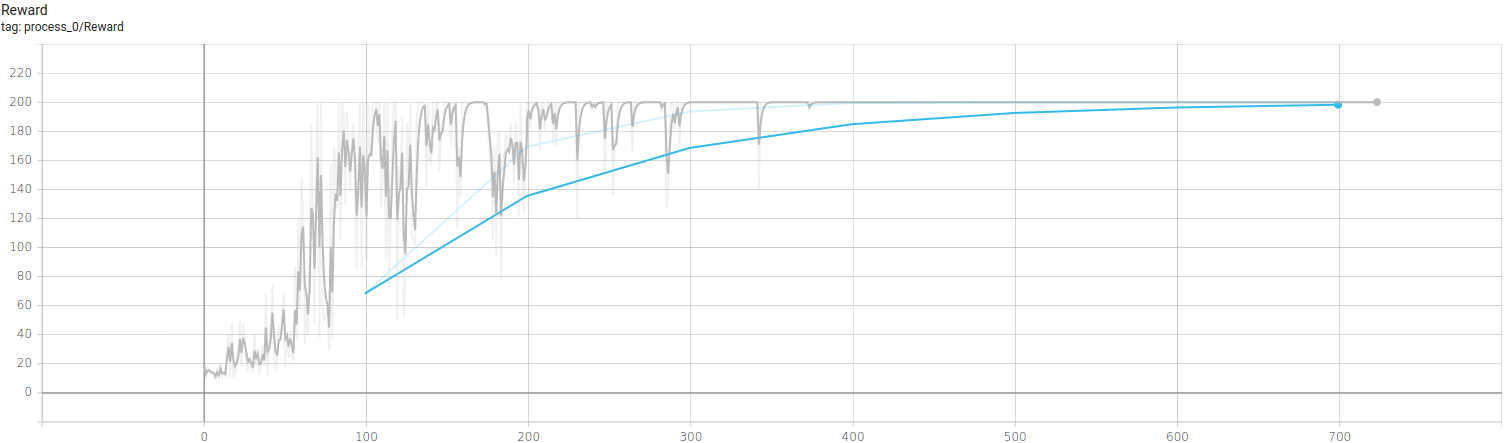
\includegraphics[width=0.8\textwidth]{images/ppo_cartpole.png}
    \caption{PPO algorithm converges completely in Cartpole environment in 400 episodes, running on 4 separate processes.}
    \label{fig:my_label}
\end{figure}

\subsection{PPG - Phasic Policy Gradient}
The advantage of sharing the same network for policy and value function is that features learnt by either of them will better optimize the other. This usually results in better generalization. However, due to competing objectives between the policy and value function, both of them are usually scaled differently. Regardless, there is still a risk that optimizing an objective may negatively affect optimization of the other. Another limitation is that it was assumed that the policy and value function can only tolerate the same number of sample reuse, which the authors of PPG showed is not necessarily true.

\begin{wrapfigure}{r}{0.25\textwidth}
    \centering
    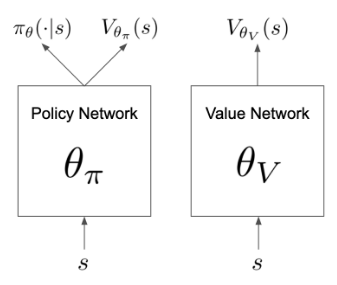
\includegraphics[width=0.25\textwidth]{images/ppg.png}
    \caption{Separated policy and value network}
\end{wrapfigure}

In PPG, the authors separated the policy from the value function. An additional auxiliary head was added to the policy, which is used to distill features from the value function into the policy. Another key contribution from PPG is the discovery that value function is more tolerant towards higher level of sample reuse compared to the policy. 

\section{Multiprocessing in Python}
Running several parallel worker instances are crucial in actor-critic methods to decorrelate data and also speeds up training time rapidly (the A3C paper has stated that running in multiple parallel processes results to almost linear improvement).

Since Python has a low-level Global Interpreter Lock (GIL), this makes multithreaded application in python more suitable towards I/O-bounded applications. Therefore, since running several worker instances is a CPU-bounded application, implementations of algorithms that require parallel worker instances have to utilize multiprocessing in python instead.

\subsection{Python Multiprocessing Library}
A3C and A2C was implemented using the Pytorch's multiprocessing library, which is a drop-in extension of python's native multiprocessing library. Several issues were ran into that made Pytorch's multiprocessing library less suitable for more complicated algorithms like PPO:
\begin{itemize}
    \item Lots of boilerplate code required for implementing various synchronization patterns. Barriers have to be manually implemented to ensure all workers in A2C are synchronized to the global network. Mutex for global variables are also implemented manually accessed by a single process at any time
\end{itemize}
\newpage
\bibliographystyle{unsrt}
\bibliography{references}

\end{document}


